A \Figref{grafico-resultados} apresenta a comparação entre a resposta simulada e a
resposta experimental do sistema. Observa-se que ambas apresentam comportamento
semelhante, indicando que o modelo identificado e modelado foi capaz de
representar adequadamente a dinâmica dominante da planta e que a estratégia de
controle proposta foi implementada com sucesso no sistema físico.

\begin{figure}[H]
\centering
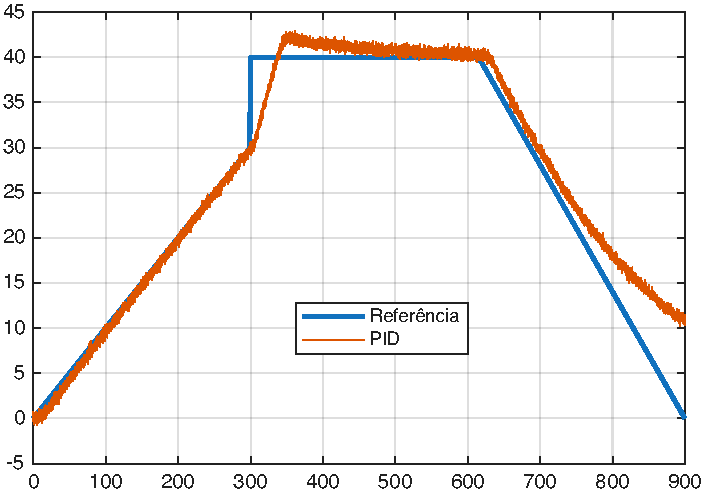
\includegraphics[width=1\linewidth]{images/Resultados.pdf}
\caption{Caption}
\figlabel{grafico-resultados}
\end{figure}

